% Informe del Taller 4 (máximo 8 páginas). Compila con pdfLaTeX o XeLaTeX.
\documentclass[10pt,a4paper]{article}
\usepackage{iftex}
\ifPDFTeX
  \usepackage[utf8]{inputenc}
  \usepackage[T1]{fontenc}
  \IfFileExists{lmodern.sty}{\usepackage{lmodern}\usepackage{microtype}}{}
  \IfFileExists{spanish.ldf}{\usepackage[spanish,es-noquoting,es-tabla,es-nodecimaldot]{babel}}{%
    \usepackage[english]{babel}%
    \addto\captionsenglish{\renewcommand{\figurename}{Figura}\renewcommand{\tablename}{Tabla}\renewcommand{\refname}{Referencias}}}
\else
  \usepackage{fontspec}
  \usepackage{polyglossia}
  \setdefaultlanguage{spanish}
  \gappto\captionsspanish{\renewcommand{\tablename}{Tabla}}
  \usepackage{microtype}
\fi
\usepackage[margin=1.9cm]{geometry}
\usepackage{amsmath,amssymb,graphicx,booktabs,array,float,xcolor}
\usepackage[font=small,labelfont=bf]{caption}
\usepackage{enumitem}
\usepackage[hidelinks]{hyperref}
\graphicspath{{../figuras/}{figuras/}}
\setlist{itemsep=0.1em,topsep=0.2em}
\setlength{\parskip}{0.3em}
\setlength{\emergencystretch}{3em}

\title{\textbf{Comparación experimental de GA, ACO, PSO, ascenso de colinas y temple simulado en el problema del viajante}}
\author{Taller 4 -- Inteligencia Artificial\\[0.35em]
\normalsize Jimmy Mill\'an, Santiago Le\'on, Natalia Orjuela\\[0.35em]
\small Repositorio: \url{https://github.com/Nataorjuela/taller4.git}}
\date{}

\begin{document}
\maketitle
\vspace{-2.5em}
\begin{abstract}
Se comparan cinco metaheurísticas sobre el TSP euclidiano con $n\in\{20,50,100\}$ ciudades (5 instancias por tamaño, 30 ejecuciones independientes por combinación),
bajo un presupuesto idéntico de evaluaciones de la función objetivo (10\,000, 30\,000 y 60\,000 FEs) y semillas emparejadas. ACO obtuvo las rutas más cortas y más estables en
todos los tamaños (error mediano 0{,}00/0{,}66/2{,}66\,\%); SA ocupó el segundo lugar en el ranking global para $n=50$ y $n=100$; HC fue el más rápido (0{,}06\,s frente a 5{,}23\,s de ACO con $n=100$);
PSO con claves aleatorias presentó los errores más altos entre los métodos evaluados. La prueba de Friedman rechazó la igualdad en los tres tamaños ($p<10^{-16}$), con un tamaño del efecto creciente
($W=0{,}63\to0{,}92$). No existe un único algoritmo que sea mejor en todos los criterios: ACO obtuvo la mejor calidad, HC los menores tiempos de ejecución y GA el menor consumo de memoria medido para $n=50$ y $n=100$.
\end{abstract}

\section{Metodología}
\textbf{Problema.} Dadas $n$ ciudades con coordenadas uniformes en $[0,100]^2$, se minimiza $f(\pi)=\sum_{k=1}^{n-1}d_{\pi_k\pi_{k+1}}+d_{\pi_n\pi_1}$ con $d_{ij}$ euclidiana y $\pi$ una permutación.
Todas las implementaciones usan la misma matriz de distancias y la misma función objetivo, centralizadas en un objeto \texttt{Evaluador} que cuenta las FEs, conserva la mejor solución histórica
y registra el historial (FEs, mejor costo). Ningún algoritmo puede exceder el presupuesto.

\textbf{Algoritmos y codificación} (Tabla~\ref{tab:alg}). HC y SA utilizan el mismo generador de vecinos basado en 2-opt. Este movimiento elimina las aristas $(a,b)$ y $(c,d)$ de la ruta y las reemplaza por $(a,c)$ y $(b,d)$. Así, el cambio de costo se calcula en $O(1)$, sin recalcular la longitud de toda la ruta, mediante
$\Delta=d_{ac}+d_{bd}-d_{ab}-d_{cd}$. Cada vecino evaluado cuenta como 1 FE; se verificó que $\Delta$ coincide con el cambio obtenido al recalcular $f$.
\begin{table}[H]\centering\small
\begin{tabular}{>{\raggedright}p{1.1cm}>{\raggedright}p{2.6cm}>{\raggedright}p{6.7cm}>{\raggedright\arraybackslash}p{4.6cm}}
\toprule
Alg. & Representación & Operadores & Parámetros (fase piloto)\\
\midrule
GA & permutación & torneo, cruce OX, mutación por inversión, elitismo & $P=50$, $k=3$, $p_c=0{,}9$, $p_m=0{,}3$, élite 2\\
ACO & ruta construida & Ant System elitista: cada paso prefiere caminos con más señal acumulada y ciudades cercanas; luego evapora señal vieja y refuerza las mejores rutas & $m=n$, $\alpha=1$, $\beta=2$, $\rho=0{,}3$, $e=5$\\
PSO & claves aleatorias, ruta $=\operatorname{argsort}(\mathbf x)$ & $\mathbf v\leftarrow w\mathbf v+c_1\mathbf r_1(\mathbf p-\mathbf x)+c_2\mathbf r_2(\mathbf g-\mathbf x)$ & $S=50$, $w=0{,}729$, $c_{1,2}=1{,}494$, $v_{\max}=0{,}5$\\
HC & permutación & vecino 2-opt aleatorio; se acepta si mejora; reinicio tras paciencia & paciencia $=2\cdot n(n-1)/2$\\
SA & permutación & mismo 2-opt; Metropolis $e^{-\Delta/T}$; $T_0=-\bar\Delta/\ln p_0$; $T_{k+1}=\alpha T_k$, $\alpha=r^{1/K}$ & $p_0=0{,}2$, $r=0{,}01$\\
\bottomrule
\end{tabular}
\caption{Algoritmos, codificación y parámetros. Los parámetros se fijaron en una fase piloto con instancias separadas (semillas 901--903, $n=50$).}\label{tab:alg}
\end{table}

\textbf{Protocolo.} Instancias con semillas públicas 101--105; 30 repeticiones por algoritmo, tamaño e instancia (2250 corridas; 450 adicionales para el híbrido).
La semilla de cada corrida depende de (2026, $n$, instancia, repetición) y es la misma para todos los algoritmos, lo que permite pruebas emparejadas.
El tiempo se mide con \texttt{perf\_counter} solo alrededor del algoritmo; la memoria pico con \texttt{tracemalloc} en una segunda pasada con la misma semilla
(repeticiones 0--4), porque \texttt{tracemalloc} ralentiza el código de forma desigual entre algoritmos. Todo se ejecutó en el mismo equipo (2 procesos).
La configuración completa está en \texttt{configuracion.json}.

\textbf{Métricas.} $f^\ast$ = mejor valor encontrado por cualquier algoritmo en todas las corridas de la instancia. Error$_r=100(f_r-f^\ast)/f^\ast$; éxito = \% de corridas con error $\le1\text{\%}$ ($R=30$ por instancia);
mejora $=100(f_{\text{inicial}}-f_r)/f_{\text{inicial}}$. Las curvas de convergencia se evalúan en 50 puntos comunes de FEs antes de promediar.
Se aplica Friedman por tamaño (150 bloques) con $W$ de Kendall, y post hoc de Wilcoxon pareado con corrección de Holm y correlación biserial de rangos.

\section{Resultados}
\subsection{Eficiencia computacional y escalabilidad}
\begin{figure}[H]\centering
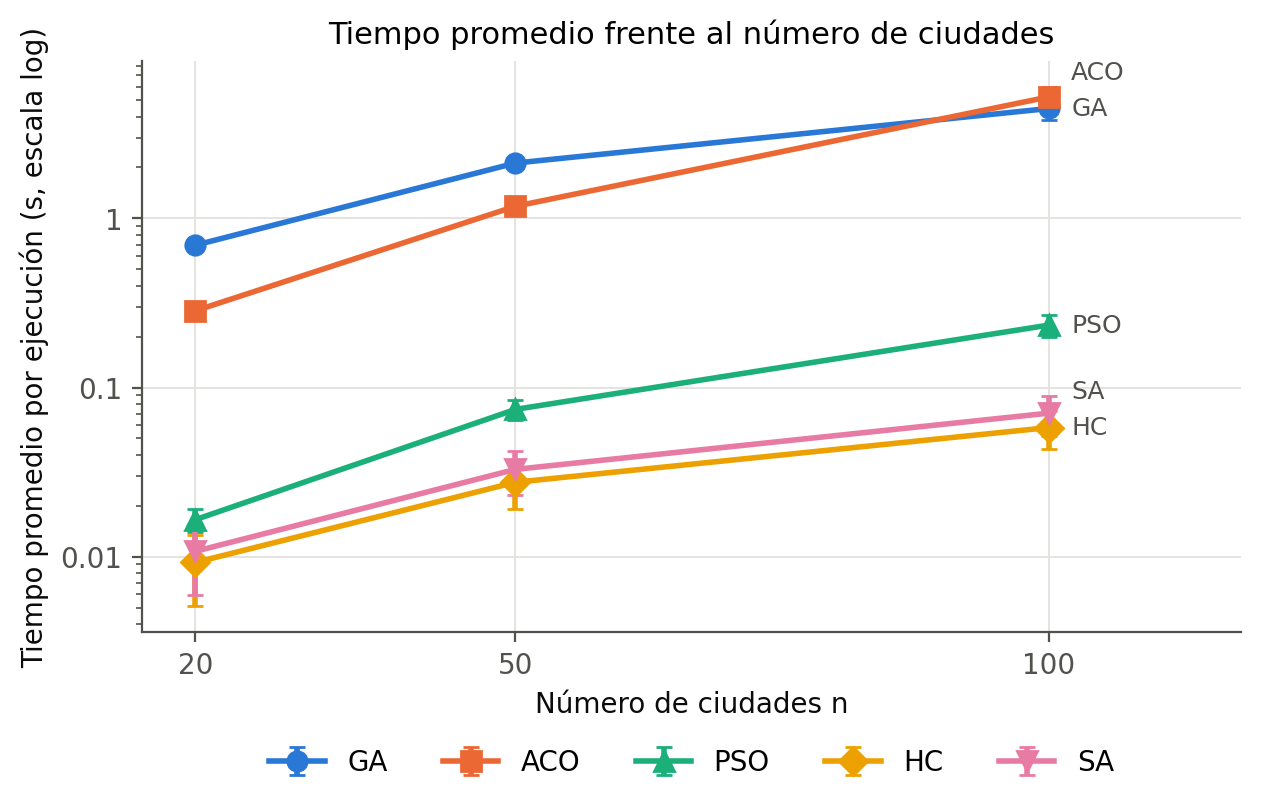
\includegraphics[width=0.49\linewidth]{fig3a_tiempo_vs_n.png}\hfill
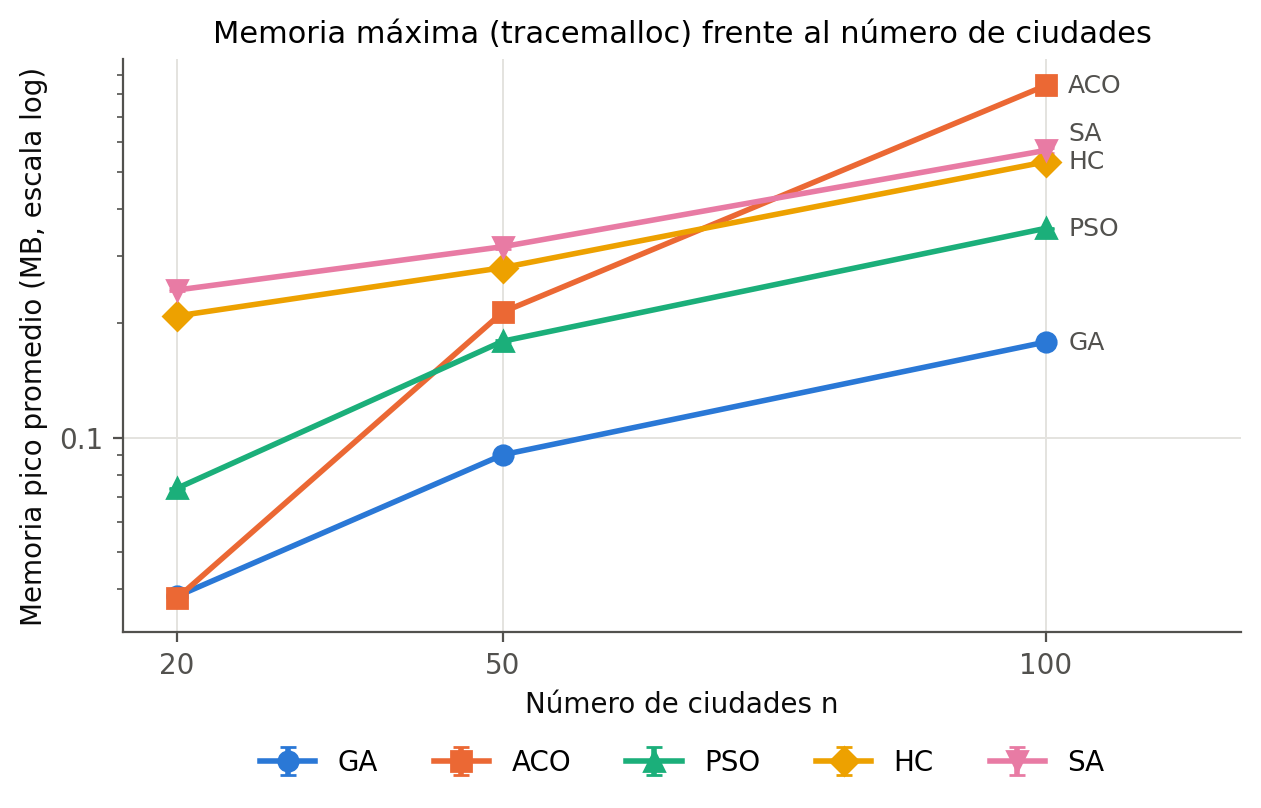
\includegraphics[width=0.49\linewidth]{fig3b_memoria_vs_n.png}
\caption{Tiempo promedio por corrida y memoria pico (\texttt{tracemalloc}) frente a $n$ (escala log; barras: $\pm1$ desviación).}\label{fig:tm}
\end{figure}
\begin{table}[H]\centering\small
\begin{tabular}{clrrrrrr}
\toprule
$n$ & Alg. & tiempo (s) & ms/1000 FEs & memoria (MB) & éxito (\%) & FEs al 1\% (med.) & llegaron \\
\midrule
20 & GA & 0{,}694 & 69{,}4 & 0{,}038 & 36{,}0 & 3\,488 & 54/150 \\
 & ACO & 0{,}284 & 28{,}4 & 0{,}038 & 99{,}3 & 242 & 149/150 \\
 & PSO & 0{,}017 & 1{,}7 & 0{,}074 & 0{,}7 & 3\,417 & 1/150 \\
 & HC & 0{,}009 & 0{,}9 & 0{,}209 & 73{,}3 & 3\,076 & 110/150 \\
 & SA & 0{,}011 & 1{,}1 & 0{,}245 & 70{,}7 & 3\,324 & 106/150 \\
\midrule
50 & GA & 2{,}124 & 70{,}8 & 0{,}090 & 2{,}0 & 22\,710 & 3/150 \\
 & ACO & 1{,}179 & 39{,}3 & 0{,}214 & 66{,}0 & 7\,713 & 99/150 \\
 & PSO & 0{,}074 & 2{,}5 & 0{,}180 & 0{,}0 & -- & 0/150 \\
 & HC & 0{,}028 & 0{,}9 & 0{,}280 & 2{,}7 & 11\,162 & 4/150 \\
 & SA & 0{,}033 & 1{,}1 & 0{,}318 & 16{,}0 & 18\,560 & 24/150 \\
\midrule
100 & GA & 4{,}463 & 74{,}4 & 0{,}179 & 0{,}0 & -- & 0/150 \\
 & ACO & 5{,}228 & 87{,}1 & 0{,}845 & 17{,}3 & 34\,784 & 26/150 \\
 & PSO & 0{,}234 & 3{,}9 & 0{,}356 & 0{,}0 & -- & 0/150 \\
 & HC & 0{,}058 & 1{,}0 & 0{,}532 & 0{,}0 & -- & 0/150 \\
 & SA & 0{,}071 & 1{,}2 & 0{,}570 & 4{,}0 & 53\,696 & 6/150 \\
\bottomrule
\end{tabular}

\caption{Tiempo, memoria, tasa de éxito y FEs necesarias para error $\le1\text{\%}$ (mediana entre las corridas que llegaron; ``llegaron'' de 150).}\label{tab:ef}
\end{table}
HC y SA presentan los menores tiempos de ejecución; para $n=100$, sus tiempos son aproximadamente 0{,}06 y 0{,}07\,s, respectivamente. Su bajo costo por FE ($\approx1$\,ms/1000 FEs) se relaciona con la evaluación incremental $O(1)$ de los movimientos 2-opt.
En cambio, el tiempo de ACO aumenta más al crecer $n$ (28$\to$87\,ms/1000 FEs), debido al proceso de construcción de rutas, cuyo costo es $O(n^2)$, y al uso de matrices $n\times n$, que también inciden en su mayor consumo de memoria ($\times22$ de $n=20$ a $n=100$).
GA registra el menor consumo de memoria medido para $n=50$ y $n=100$ (con empate práctico entre GA y ACO en $n=20$), aunque su costo por FE ($\approx70$\,ms/1000) está dominado por operaciones en Python. Estos resultados muestran que un menor tiempo de ejecución no implica necesariamente una mejor calidad: para $n=100$, ACO alcanzó el error $\le1\text{\%}$ en 26 de 150 ejecuciones, frente a 6 de 150 para SA.

\subsection{Convergencia, calidad y estabilidad}
\begin{figure}[H]\centering
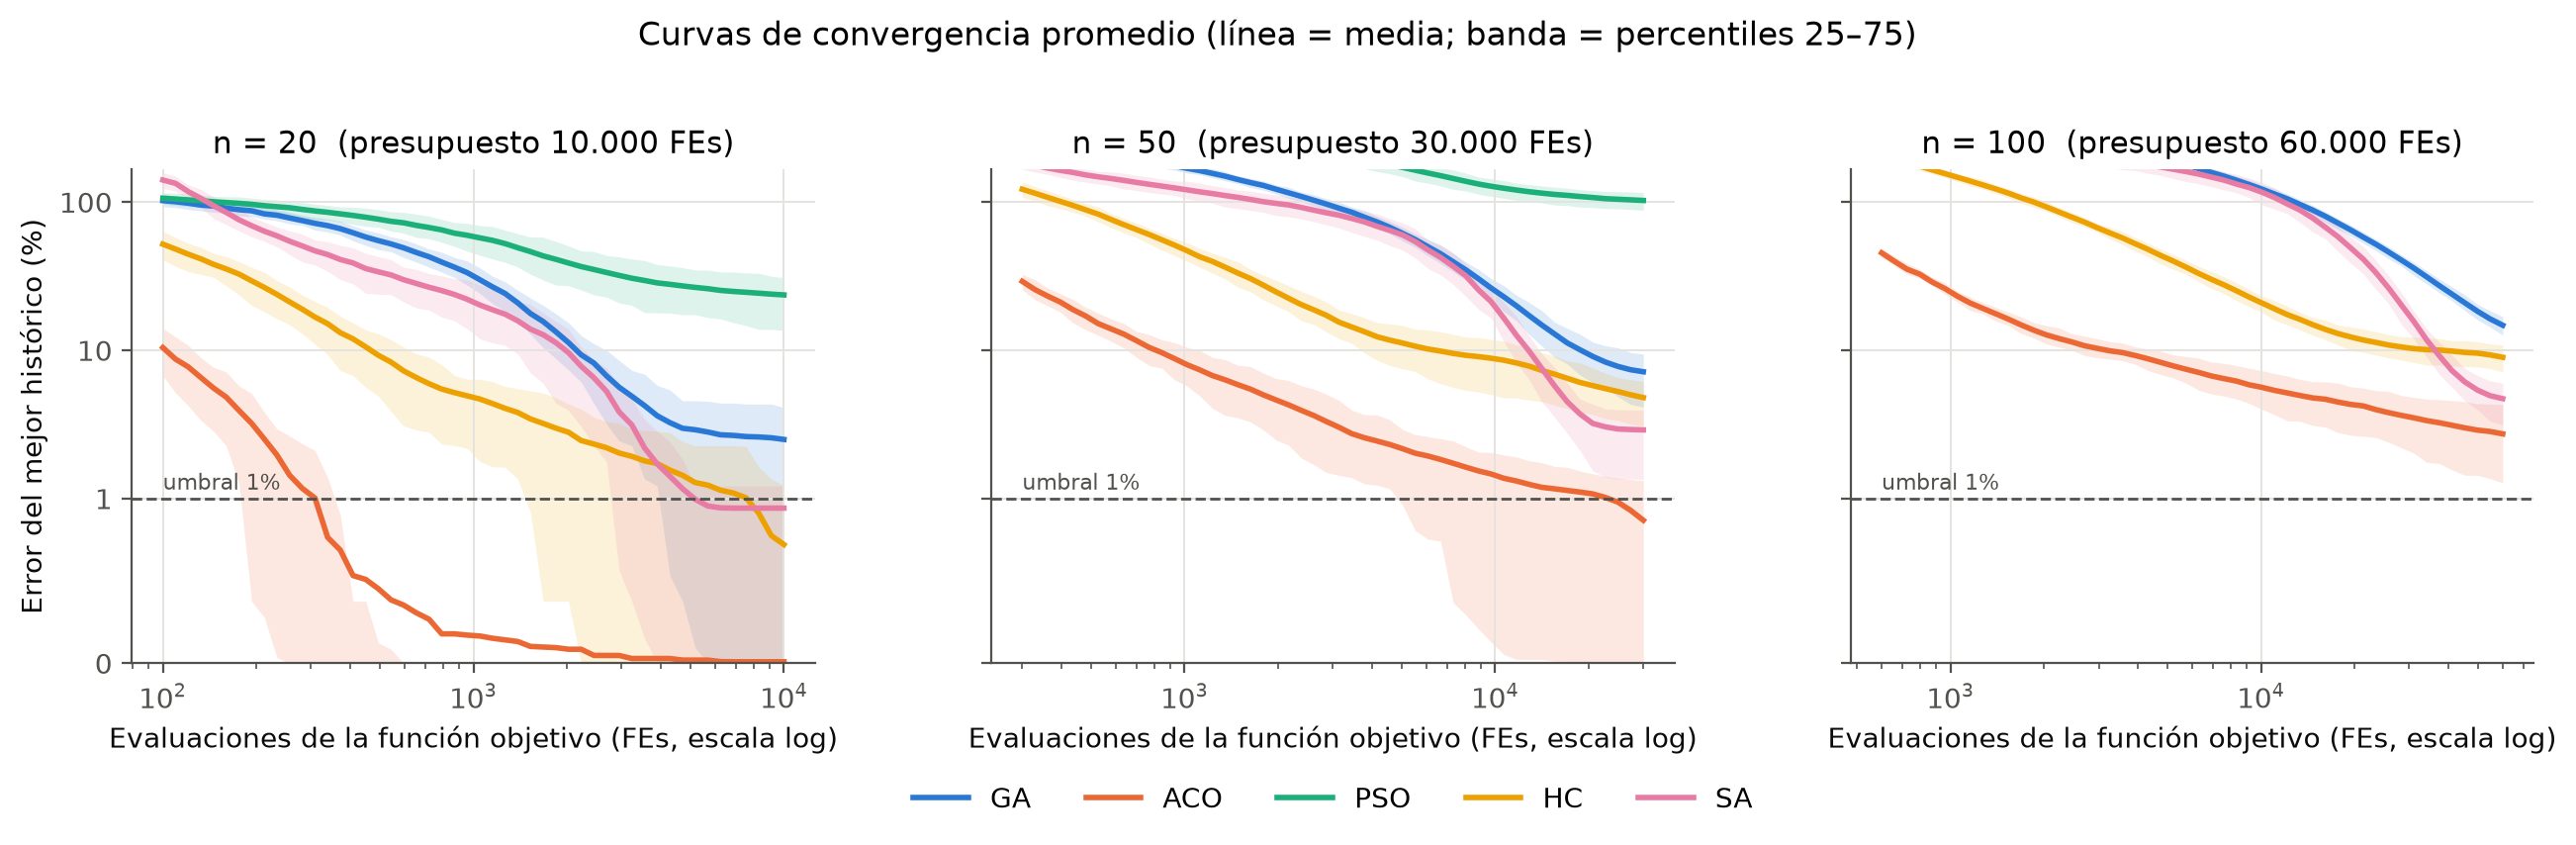
\includegraphics[width=\linewidth]{fig4a_convergencia.png}
\caption{Error del mejor histórico frente a FEs (media y percentiles 25--75 de 150 corridas; ejes logarítmicos, eje $y$ lineal en $[0,1]$).}\label{fig:conv}
\end{figure}
\begin{figure}[H]\centering
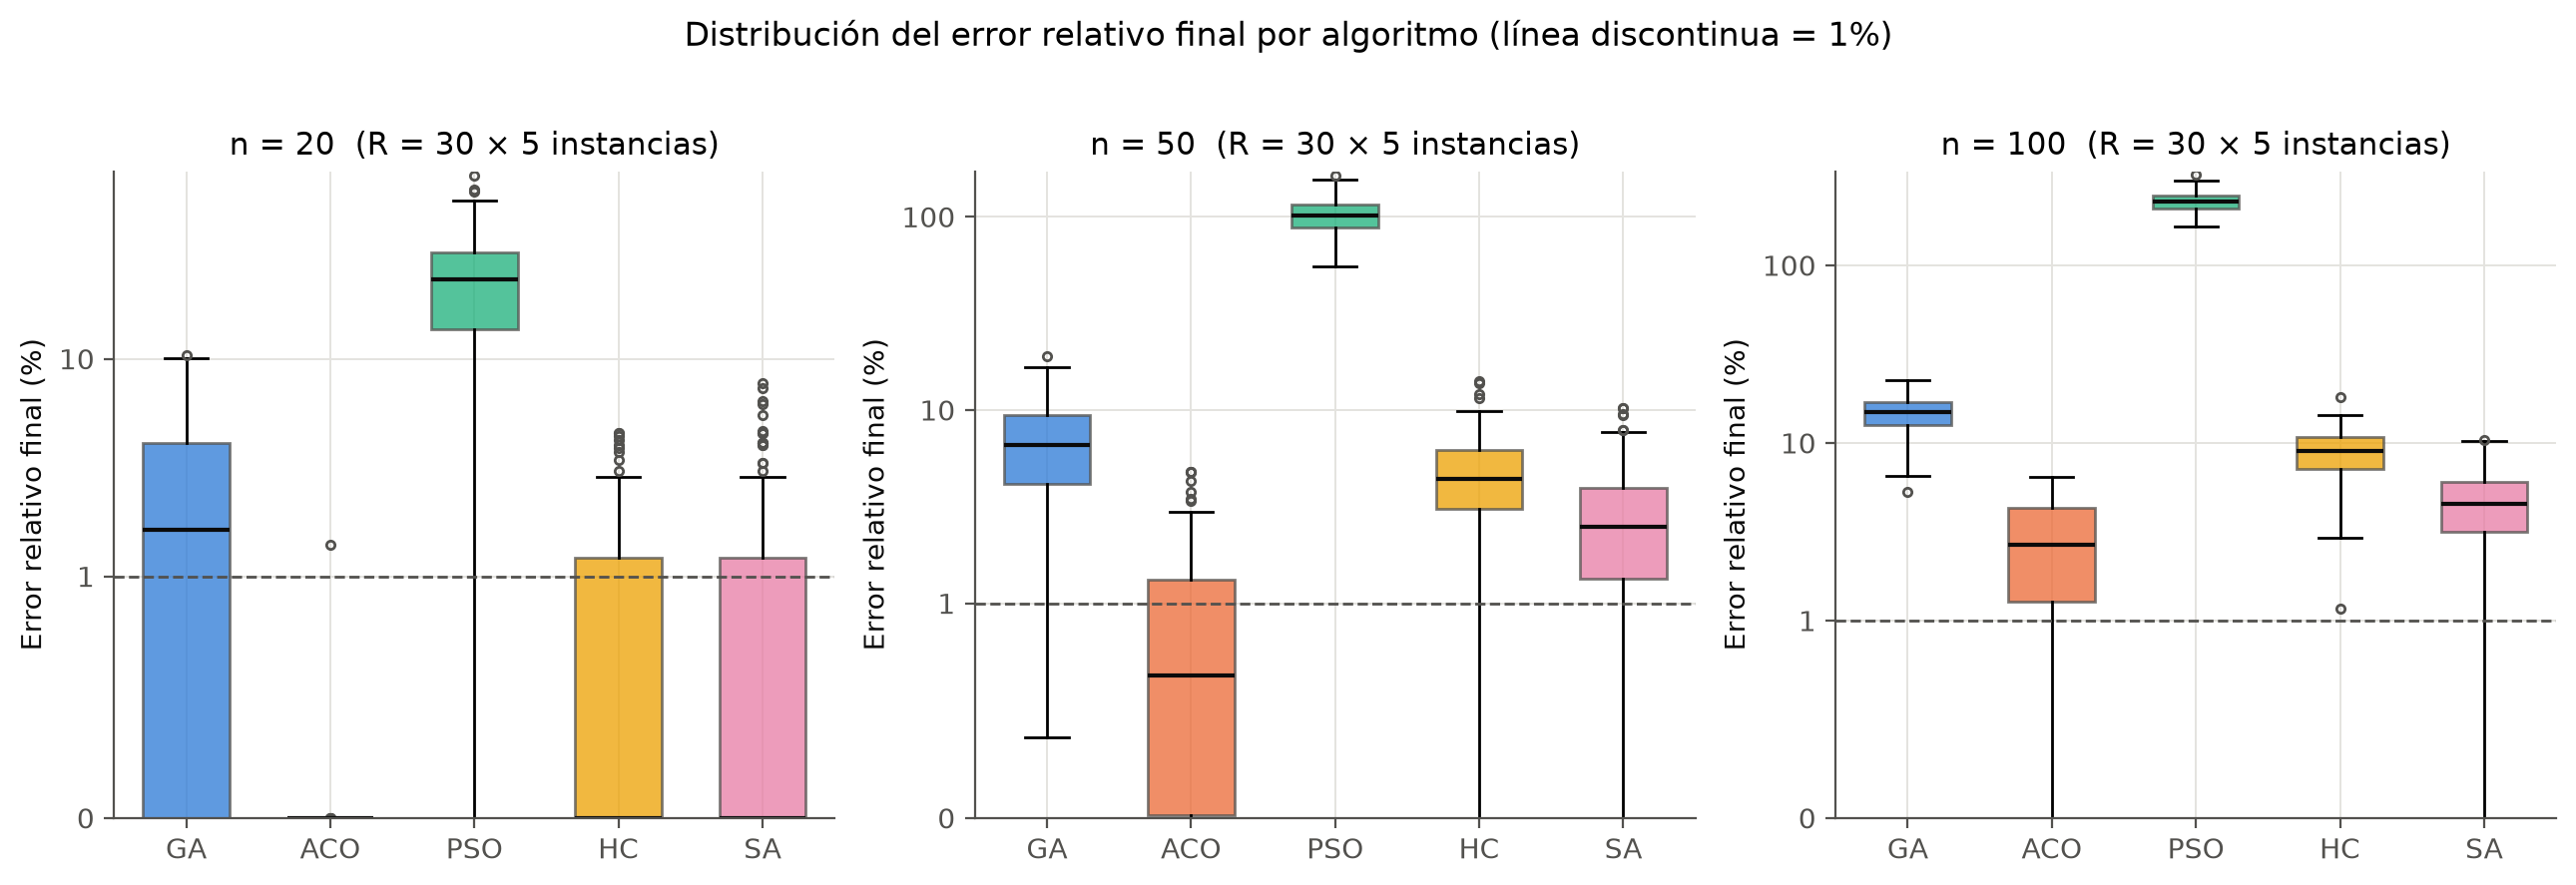
\includegraphics[width=\linewidth]{fig4b_cajas_error.png}
\caption{Diagramas de caja del error relativo final (150 corridas por algoritmo y tamaño).}\label{fig:cajas}
\end{figure}
\begin{table}[H]\centering\small
\begin{tabular}{clrrrrrrr}
\toprule
$n$ & Alg. & mejor & media & mediana & desv.$^\dagger$ & RIC & éxito (\%) & mejora (\%) \\
\midrule
20 & GA & 0{,}00 & 2{,}51 & 1{,}63 & 2{,}14 & 4{,}12 & 36{,}0 & 61{,}7 \\
 & ACO & 0{,}00 & 0{,}01 & 0{,}00 & 0{,}05 & 0{,}00 & 99{,}3 & 40{,}9 \\
 & PSO & 0{,}00 & 23{,}67 & 23{,}10 & 13{,}07 & 17{,}30 & 0{,}7 & 53{,}8 \\
 & HC & 0{,}00 & 0{,}72 & 0{,}00 & 0{,}89 & 1{,}22 & 73{,}3 & 62{,}3 \\
 & SA & 0{,}00 & 0{,}94 & 0{,}00 & 0{,}98 & 1{,}22 & 70{,}7 & 62{,}2 \\
\midrule
50 & GA & 0{,}37 & 7{,}17 & 6{,}61 & 3{,}70 & 5{,}31 & 2{,}0 & 76{,}3 \\
 & ACO & 0{,}00 & 0{,}87 & 0{,}66 & 0{,}62 & 1{,}31 & 66{,}0 & 55{,}8 \\
 & PSO & 55{,}13 & 102{,}71 & 101{,}72 & 19{,}69 & 27{,}99 & 0{,}0 & 55{,}5 \\
 & HC & 0{,}00 & 4{,}80 & 4{,}41 & 2{,}36 & 3{,}09 & 2{,}7 & 76{,}8 \\
 & SA & 0{,}00 & 2{,}91 & 2{,}50 & 2{,}06 & 2{,}61 & 16{,}0 & 77{,}2 \\
\midrule
100 & GA & 5{,}29 & 14{,}78 & 14{,}91 & 3{,}30 & 4{,}22 & 0{,}0 & 82{,}2 \\
 & ACO & 0{,}00 & 2{,}73 & 2{,}66 & 0{,}89 & 3{,}04 & 17{,}3 & 63{,}5 \\
 & PSO & 165{,}26 & 230{,}27 & 228{,}01 & 24{,}07 & 39{,}56 & 0{,}0 & 48{,}6 \\
 & HC & 1{,}17 & 8{,}98 & 8{,}97 & 2{,}52 & 3{,}72 & 0{,}0 & 83{,}1 \\
 & SA & 0{,}00 & 4{,}72 & 4{,}56 & 2{,}19 & 2{,}87 & 4{,}0 & 83{,}8 \\
\bottomrule
\end{tabular}

\caption{Error relativo final (\%). $^\dagger$Desviación estándar dentro de cada instancia, promediada. El costo absoluto (mejor, media, mediana y desviación) por instancia está en \texttt{resultados/tabla\_rendimiento\_por\_instancia.csv}.}\label{tab:rend}
\end{table}
ACO encuentra buenas rutas desde las primeras etapas, gracias a la visibilidad $1/d$, y conserva una ventaja durante gran parte del presupuesto (Fig.~\ref{fig:conv}). HC mejora rápidamente al inicio, pero después tiende a estancarse.
Al principio, SA explora más alternativas debido a la temperatura; conforme esta disminuye, la búsqueda se concentra en mejorar las soluciones encontradas. Para $n=50$ y $n=100$, SA obtiene mejores resultados finales que HC. GA continúa encontrando mejoras cerca del final del presupuesto, especialmente para $n=100$ (mejor solución en la FE mediana del 98\,\%), lo que sugiere que podría beneficiarse de un presupuesto mayor.
PSO presenta dificultades para mejorar las rutas: pequeños cambios en su vector continuo de claves no necesariamente generan cambios pequeños o favorables en la ruta que resulta al ordenar sus componentes. La Fig.~\ref{fig:rutas} muestra las rutas de la corrida mediana: ACO, SA y HC no presentan cruces, mientras que PSO presenta varios.
\begin{figure}[H]\centering
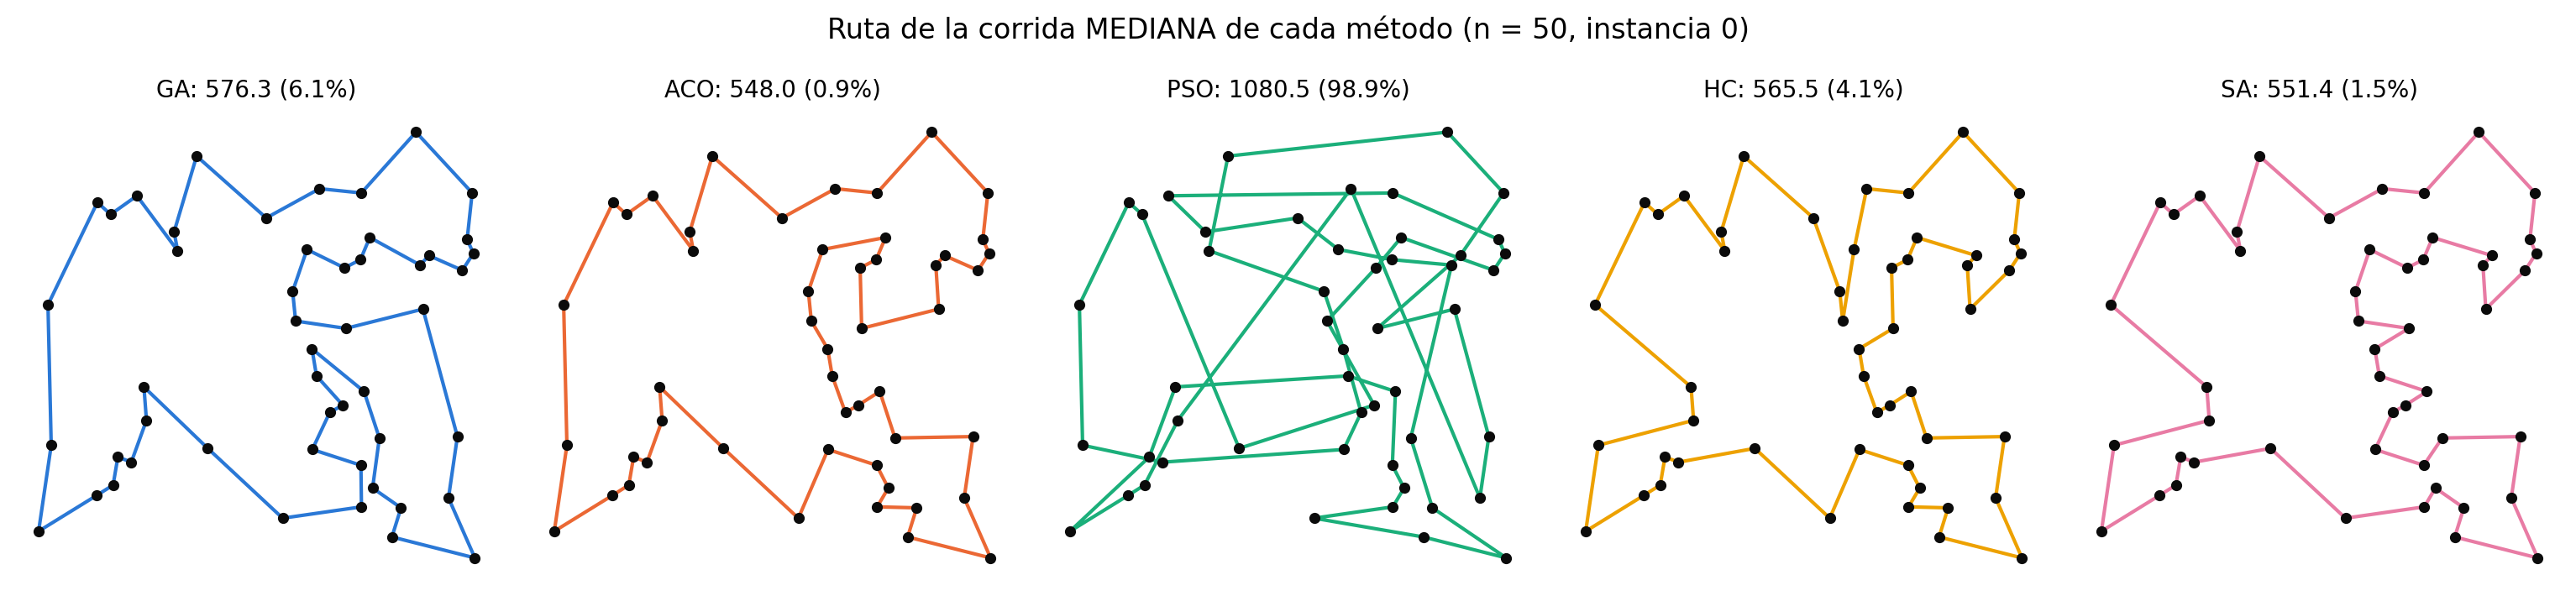
\includegraphics[width=\linewidth]{fig4d_rutas.png}
\caption{Ruta de la corrida mediana de cada método en la instancia 0 con $n=50$ (entre paréntesis, error respecto a $f^\ast$).}\label{fig:rutas}
\end{figure}

\subsection{Análisis estadístico y ranking}
\begin{table}[H]\centering\small
\begin{tabular}{rrrrrrrrr}
\toprule
$n$ & $\chi^2_F$ & $p$ & $W$ & $\bar R$ GA & $\bar R$ ACO & $\bar R$ PSO & $\bar R$ HC & $\bar R$ SA \\
\midrule
20 & 379{,}6 & $<10^{-16}$ & 0{,}633 & 3{,}31 & 1{,}84 & 4{,}95 & 2{,}31 & 2{,}58 \\
\midrule
50 & 467{,}4 & $<10^{-16}$ & 0{,}779 & 3{,}50 & 1{,}31 & 5{,}00 & 3{,}02 & 2{,}17 \\
\midrule
100 & 549{,}5 & $<10^{-16}$ & 0{,}916 & 3{,}93 & 1{,}26 & 5{,}00 & 2{,}93 & 1{,}88 \\
\bottomrule
\end{tabular}

\caption{Friedman ($N=150$, $k=5$) y rangos promedio (1 = mejor).}\label{tab:fried}
\end{table}
\begin{table}[H]\centering\footnotesize
\begin{tabular}{llll}
\toprule
Par & $n=20$ & $n=50$ & $n=100$ \\
\midrule
GA vs ACO & ACO (0{,}88; $<10^{-4}$) & ACO (0{,}99; $<10^{-4}$) & ACO (1{,}00; $<10^{-4}$) \\
GA vs PSO & GA ($-$0{,}99; $<10^{-4}$) & GA ($-$1{,}00; $<10^{-4}$) & GA ($-$1{,}00; $<10^{-4}$) \\
GA vs HC & HC (0{,}70; $<10^{-4}$) & HC (0{,}54; $<10^{-4}$) & HC (0{,}96; $<10^{-4}$) \\
GA vs SA & SA (0{,}63; $<10^{-4}$) & SA (0{,}85; $<10^{-4}$) & SA (1{,}00; $<10^{-4}$) \\
ACO vs PSO & ACO ($-$1{,}00; $<10^{-4}$) & ACO ($-$1{,}00; $<10^{-4}$) & ACO ($-$1{,}00; $<10^{-4}$) \\
ACO vs HC & ACO ($-$0{,}51; $<10^{-4}$) & ACO ($-$0{,}96; $<10^{-4}$) & ACO ($-$1{,}00; $<10^{-4}$) \\
ACO vs SA & ACO ($-$0{,}63; $<10^{-4}$) & ACO ($-$0{,}77; $<10^{-4}$) & ACO ($-$0{,}66; $<10^{-4}$) \\
PSO vs HC & HC (1{,}00; $<10^{-4}$) & HC (1{,}00; $<10^{-4}$) & HC (1{,}00; $<10^{-4}$) \\
PSO vs SA & SA (1{,}00; $<10^{-4}$) & SA (1{,}00; $<10^{-4}$) & SA (1{,}00; $<10^{-4}$) \\
HC vs SA & HC ($-$0{,}21; 0{,}0258) & SA (0{,}65; $<10^{-4}$) & SA (0{,}92; $<10^{-4}$) \\
\bottomrule
\end{tabular}

\caption{Wilcoxon pareado con Holm: ganador (biserial de rangos; $p$ ajustado). Todas las diferencias son significativas a $\alpha=0{,}05$.}\label{tab:ph}
\end{table}
\begin{table}[H]\centering\small
\begin{tabular}{clccccrrr}
\toprule
$n$ & Alg. & calidad & estab. & converg. & global & $\bar R$ & desv. error & AUC \\
\midrule
20 & ACO & 1 & 1 & 1 & \textbf{1} & 1{,}84 & 0{,}05 & 2{,}5 \\
 & HC & 2 & 2 & 2 & \textbf{2} & 2{,}31 & 0{,}89 & 22{,}9 \\
 & SA & 3 & 3 & 3 & \textbf{3} & 2{,}58 & 0{,}98 & 64{,}2 \\
 & GA & 4 & 4 & 4 & \textbf{4} & 3{,}31 & 2{,}14 & 79{,}1 \\
 & PSO & 5 & 5 & 5 & \textbf{5} & 4{,}95 & 13{,}07 & 120{,}2 \\
\midrule
50 & ACO & 1 & 1 & 1 & \textbf{1} & 1{,}31 & 0{,}62 & 12{,}6 \\
 & SA & 2 & 2 & 3 & \textbf{2} & 2{,}17 & 2{,}06 & 157{,}7 \\
 & HC & 3 & 3 & 2 & \textbf{3} & 3{,}02 & 2{,}36 & 65{,}9 \\
 & GA & 4 & 4 & 4 & \textbf{4} & 3{,}50 & 3{,}70 & 208{,}0 \\
 & PSO & 5 & 5 & 5 & \textbf{5} & 5{,}00 & 19{,}69 & 389{,}0 \\
\midrule
100 & ACO & 1 & 1 & 1 & \textbf{1} & 1{,}26 & 0{,}89 & 22{,}1 \\
 & SA & 2 & 2 & 3 & \textbf{2} & 1{,}88 & 2{,}19 & 284{,}9 \\
 & HC & 3 & 3 & 2 & \textbf{3} & 2{,}93 & 2{,}52 & 120{,}9 \\
 & GA & 4 & 4 & 4 & \textbf{4} & 3{,}93 & 3{,}30 & 363{,}7 \\
 & PSO & 5 & 5 & 5 & \textbf{5} & 5{,}00 & 24{,}07 & 726{,}5 \\
\bottomrule
\end{tabular}

\caption{Ranking por calidad (rango de Friedman), estabilidad (desviación del error dentro de instancia) y velocidad de convergencia (área bajo la curva de error en $\log$ FEs; AUC).}\label{tab:rank}
\end{table}
Las pruebas estadísticas muestran diferencias significativas entre los algoritmos en los tres tamaños evaluados. Además, estas diferencias se hacen más marcadas a medida que aumenta el número de ciudades: el $W$ de Kendall pasa de 0{,}63 con $n=20$ a 0{,}92 con $n=100$.
La diferencia entre HC y SA es pequeña con $n=20$ (biserial $-0{,}21$, $p=0{,}026$), pero cambia a favor de SA con $n=50$ y $n=100$.

\section{Discusión}
\begin{enumerate}[leftmargin=1.2em]
\item \textbf{Menor costo y mayor estabilidad:} ACO obtuvo las rutas de menor costo y presentó la mayor estabilidad en los tres tamaños. Sus errores medianos fueron 0{,}00\,\%, 0{,}66\,\% y 2{,}66\,\% para $n=20$, $n=50$ y $n=100$, respectivamente; además, la menor variabilidad observada en sus resultados respalda esta conclusión (Tablas~\ref{tab:rend} y~\ref{tab:rank}).
\item \textbf{Error $\le1\text{\%}$ con menos FEs:} ACO fue el algoritmo que alcanzó el error $\le1\text{\%}$ con menos evaluaciones. Para 20 ciudades necesitó una mediana de 242 FEs para llegar a ese umbral, y para 50 ciudades necesitó 7.713. En 100 ciudades siguió siendo el método que alcanzó este umbral con mayor frecuencia, aunque solo lo logró en 26 de las 150 ejecuciones.
\item HC fue el algoritmo con menor tiempo de ejecución, mientras que GA presentó el menor consumo de memoria para 50 y 100 ciudades. Esto no coincide con el algoritmo de mejor calidad, ya que ACO produjo las mejores soluciones, pero tuvo un costo computacional mayor, especialmente al aumentar el número de ciudades.
\item El ranking se mantuvo relativamente estable para ACO, GA y PSO. ACO ocupó el primer lugar en todos los tamaños, GA se mantuvo cuarto y PSO quinto. El principal cambio ocurrió entre HC y SA: con 20 ciudades HC tuvo mejores resultados, pero al aumentar a 50 y 100 ciudades SA pasó a superarlo.
\item Los resultados muestran que trabajar con una población no garantiza por sí solo mejores resultados. En ACO, las hormigas comparten información mediante las feromonas y esto ayuda a orientar la búsqueda hacia rutas prometedoras. En cambio, GA necesita varias evaluaciones en cada generación y puede perder partes buenas de una ruta durante el cruce. En PSO, la representación mediante claves aleatorias tampoco permitió aprovechar bien la información de las mejores soluciones. Por otro lado, HC y SA trabajan sobre una sola solución y pueden avanzar rápidamente, aunque tienen mayor riesgo de quedar atrapados en óptimos locales.
\item Aceptar temporalmente soluciones peores puede ser útil cuando el algoritmo corre el riesgo de quedar atrapado en un óptimo local. Esto se observa en SA: al principio puede avanzar más lentamente porque explora diferentes alternativas, pero con 50 y 100 ciudades termina obteniendo mejores resultados que HC. Algo similar ocurre con la diversidad en los métodos poblacionales: puede ayudar a explorar más soluciones, pero demasiada diversidad también puede retrasar la convergencia.
\item No existe un ganador absoluto, porque la mejor opción depende de lo que se quiera priorizar. Si se necesita una respuesta rápida, HC sería una buena alternativa por su bajo tiempo de ejecución. Si se busca principalmente calidad, ACO obtuvo los mejores resultados. Para un escenario con memoria limitada, GA presentó el menor consumo medido en los problemas de 50 y 100 ciudades.
\end{enumerate}

\textbf{Amenaza a la validez.} $f^\ast$ corresponde al mejor valor encontrado durante los experimentos, pero no necesariamente al óptimo real de cada instancia. Por ello, el error relativo calculado respecto a $f^\ast$ puede subestimar la distancia al óptimo real. Además, la referencia puede favorecer al algoritmo que encontró la solución usada como $f^\ast$, un efecto especialmente relevante para ACO con $n=100$.
Los parámetros se ajustaron utilizando instancias con $n=50$ y, por tanto, podrían no ser los mejores para los otros tamaños. Asimismo, los tiempos medidos pueden depender tanto del algoritmo como de diferencias de implementación, incluido el grado de vectorización en NumPy.
\textbf{Mejoras futuras:} utilizar instancias con óptimos conocidos (TSPLIB o Concorde), ajustar los parámetros por tamaño (por ejemplo, con irace) y comparar implementaciones con niveles similares de optimización.

\textbf{Híbrido ACO + 2-opt (opcional).} La mejor hormiga de cada iteración se mejora con $5n$ propuestas 2-opt (mismas FEs totales). El híbrido supera a HC (92--96\,\% de corridas para $n\ge50$) y a SA (65--74\,\%) con $p<10^{-4}$,
pero no a ACO puro: empata con $n=20$ ($p=0{,}31$) y pierde con $n=50$ y $n=100$ (error mediano 1{,}03 vs.\ 0{,}66 y 3{,}59 vs.\ 2{,}66\,\%; $p<0{,}01$). La búsqueda local consume $5n$ FEs por iteración y reduce las iteraciones de la colonia de 600 a $\approx100$;
el híbrido fue aproximadamente 5 veces más rápido en tiempo de ejecución. Por esta razón, una comparación basada en tiempo de ejecución, en lugar de utilizar únicamente el número de FEs, podría producir resultados diferentes; estos resultados no permiten concluir que el híbrido sería necesariamente mejor con ese criterio.

\section{Conclusiones}
Una comparación entre metaheurísticas debe considerar conjuntamente la calidad de las soluciones, su estabilidad, la velocidad de convergencia y el costo computacional. En este estudio, los algoritmos se evaluaron con las mismas instancias, presupuestos de FEs y semillas, lo que permitió realizar comparaciones emparejadas.
ACO obtuvo las soluciones de mayor calidad y presentó la mayor estabilidad. HC y SA registraron los menores tiempos de ejecución; además, SA superó a HC en calidad al aumentar el problema a 50 y 100 ciudades. GA mostró un comportamiento intermedio y continuó encontrando mejoras cerca del final del presupuesto, mientras que PSO con claves aleatorias presentó los errores más altos para este problema.
En consecuencia, no hay un algoritmo que sea mejor en todos los criterios y la elección depende de cuál se quiera priorizar. Estas conclusiones se apoyan en 150 ejecuciones emparejadas por tamaño, el análisis de la variabilidad y las pruebas estadísticas, no únicamente en los valores promedio.

\end{document}
